\subsection{Franke function data}

\mia{textbf to be taken away (maybe)}

\subsubsection{Neural network}

Based on the initial search, using the \mia{fix} optimizer seems to be a good choice for the further investigation.
Furthermore, we note that the three best ones are \mia{fix}. 

\textbf{Structure}

\begin{figure}
    \centering
    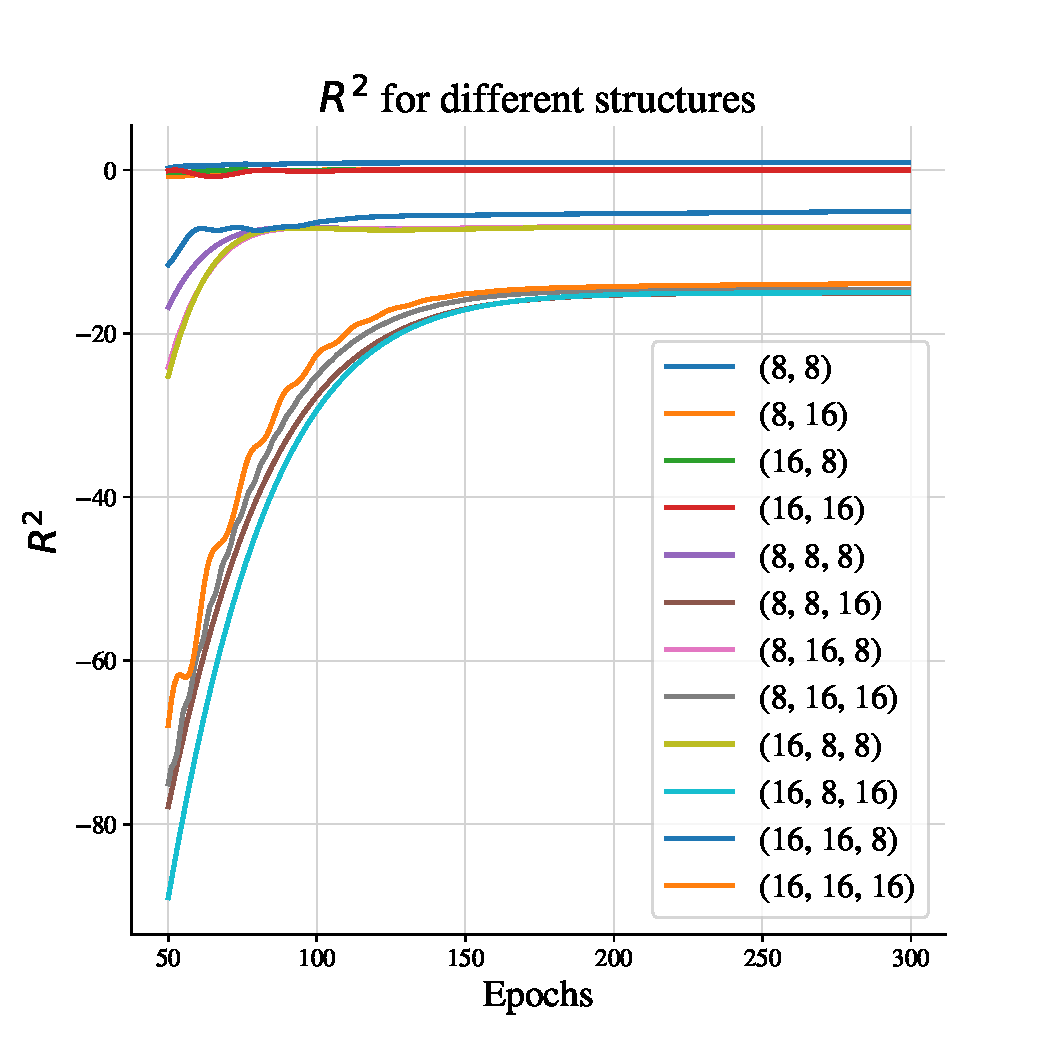
\includegraphics[width=1.0\linewidth]{project_2/figures/$R^2$ for different structures_continuous.pdf}
    \caption{$R^2$ for the neural network for different number of layers and sizes for each layer.}
    \label{fig:structure_franke}
\end{figure}

Fig. \ref{fig:structure_franke} shows the $R^2$ for models with different network structure, but otherwise the same parameters. It is interesting to notice that \mia{...}
The structure of the network dictate \mia{... smt abt the workings of structure}

\textbf{Activation functions}

\begin{figure}
    \centering
    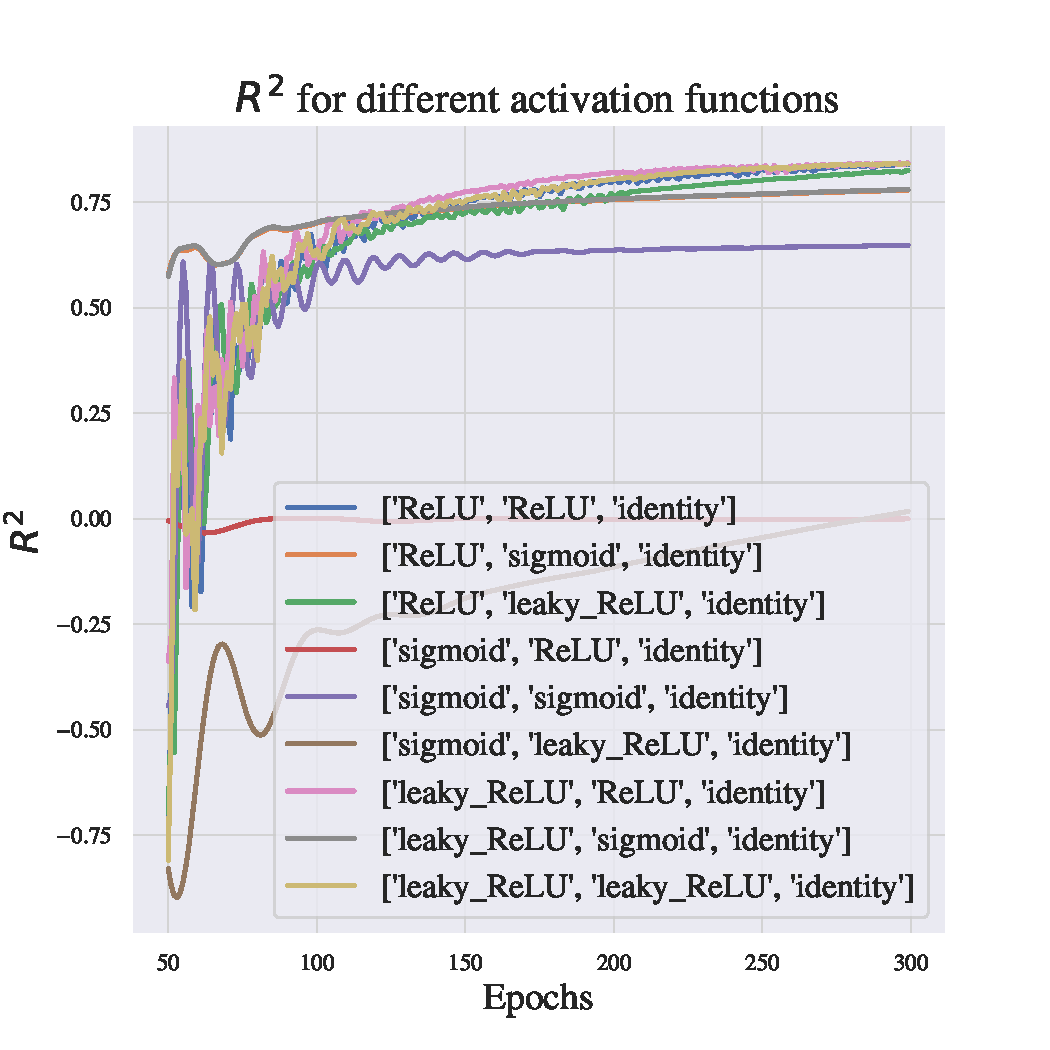
\includegraphics[width=1.0\linewidth]{project_2/figures/$R^2$ for different activation functions_continuous.pdf}
    \caption{Caption}
    \label{fig:activation_franke}
\end{figure}

Using the network structure found in the previous step, we try different activation functions for the \mia{number} hidden layers. Fig. \ref{fig:activation_franke} visualizes how the different models perform. For the final layer identity is always used as the activation function \mia{think about it...}. 
The best performing models are the ones that \mia{...}
The reason for this might be 

\textbf{Initial learning rate and batch size}

\begin{figure}
    \centering
    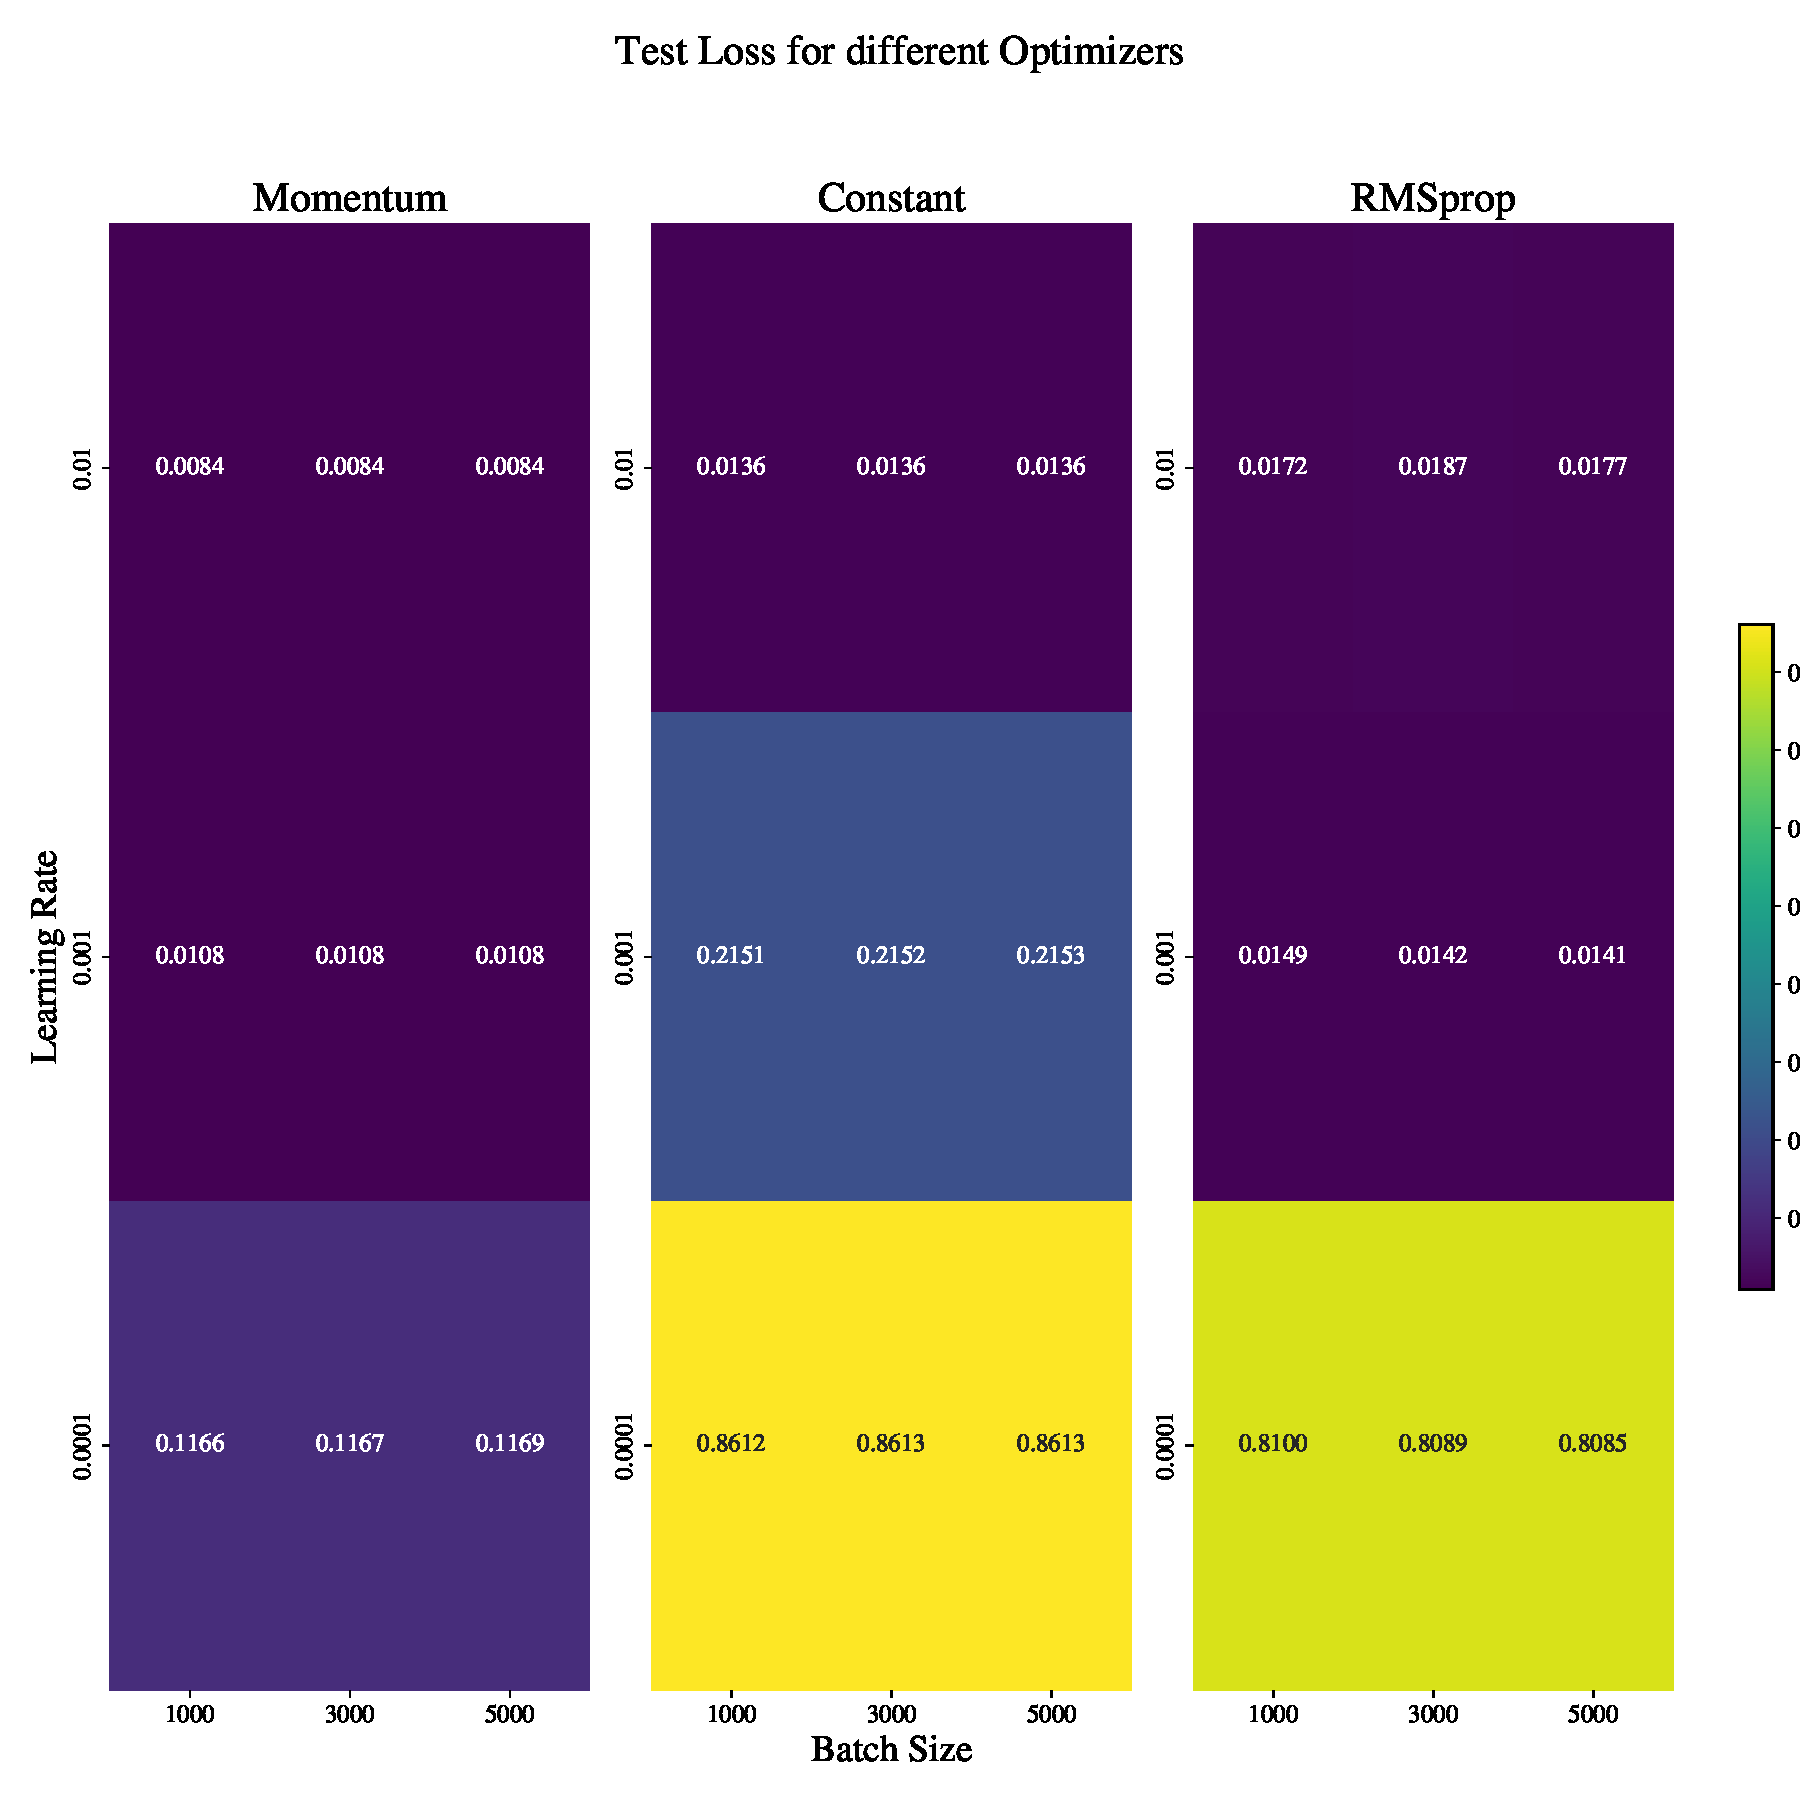
\includegraphics[width=1.0\linewidth]{project_2/figures/Loss_grid_continuous.pdf}
    \caption{Caption}
    \label{fig:grid_franke}
\end{figure}

Using \mia{...} as the network structure and \mia{...} as the activation functions, the grid search for the best combination of initial learning rate and batch size is showed in Fig. \ref{fig:grid_franke}. The three best optimizers, \mia{names}, are used. 

\textbf{The best model}

\begin{figure}
    \centering
    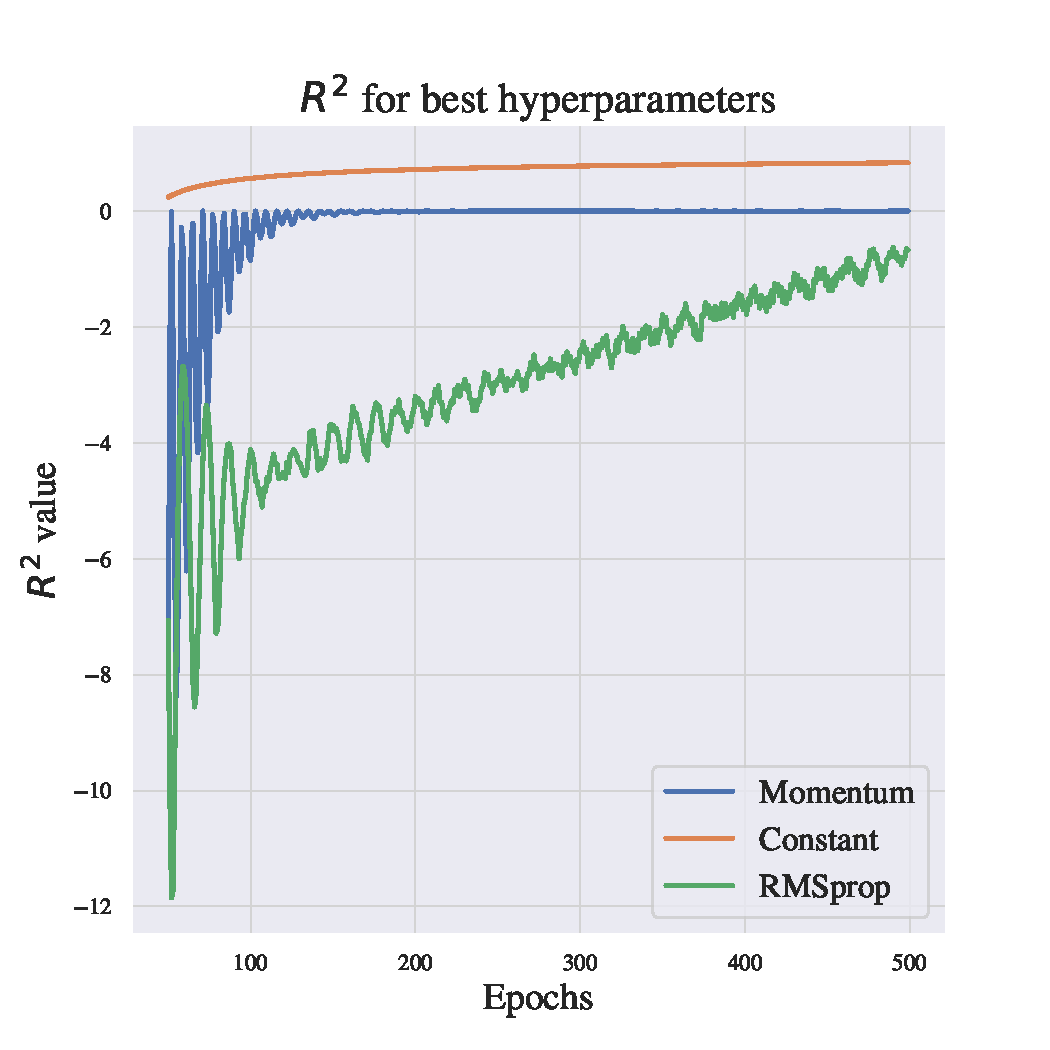
\includegraphics[width=1.0\linewidth]{project_2/figures/best_continuous.pdf}
    \caption{Caption}
    \label{fig:best_franke}
\end{figure}

Final values: 



\subsubsection{Linear regression}

Final values: 

\subsection{Breast cancer data}

\subsubsection{Neural network}


Based on the initial search, using the \mia{fix} optimizer seems to be a good choice for the further investigation.

\textbf{Structure}

\begin{figure}
    \centering
    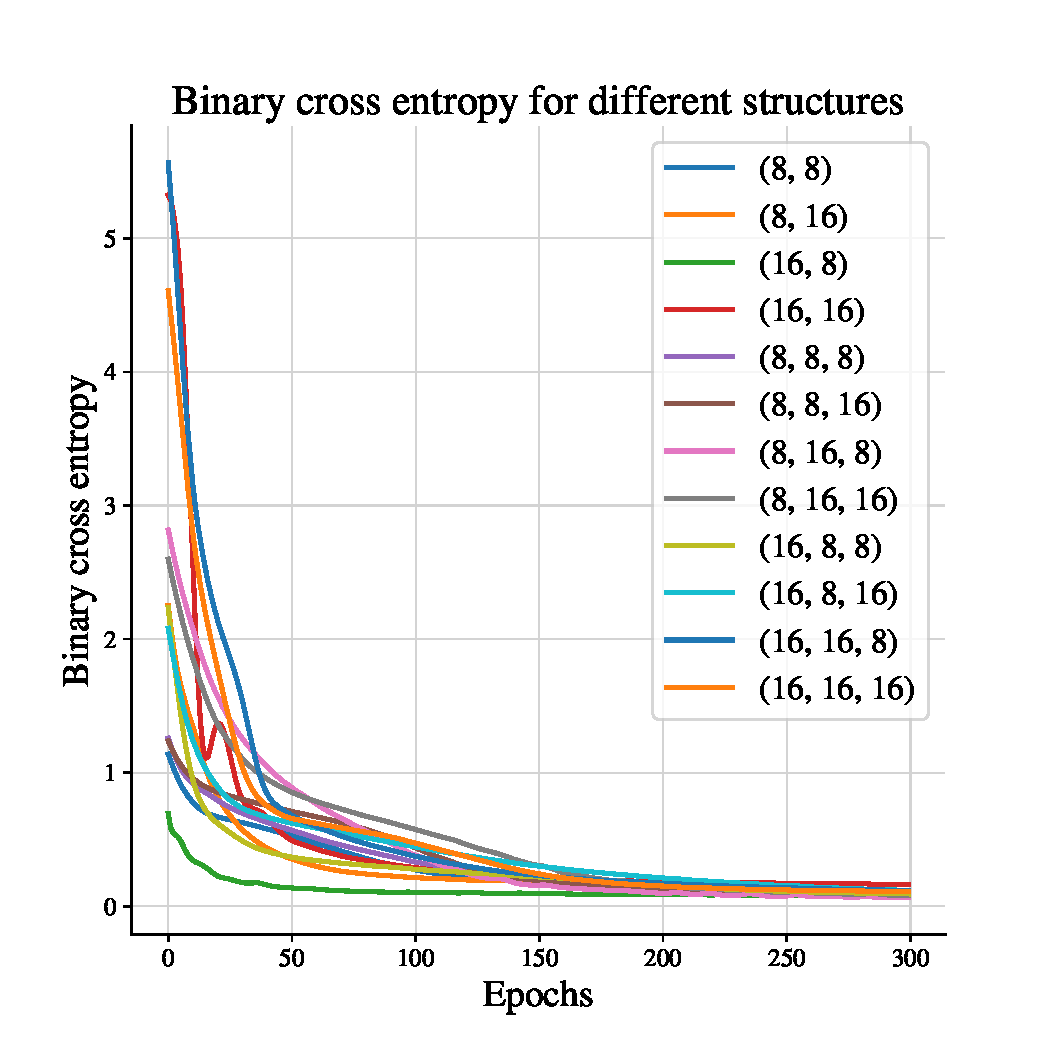
\includegraphics[width=1.0\linewidth]{project_2/figures/Binary cross entropy for different structures_classification.pdf}
    \caption{$R^2$ for the neural network for different number of layers and sizes for each layer.}
    \label{fig:structure_cancer}
\end{figure}

\textbf{Activation functions}

\begin{figure}
    \centering
    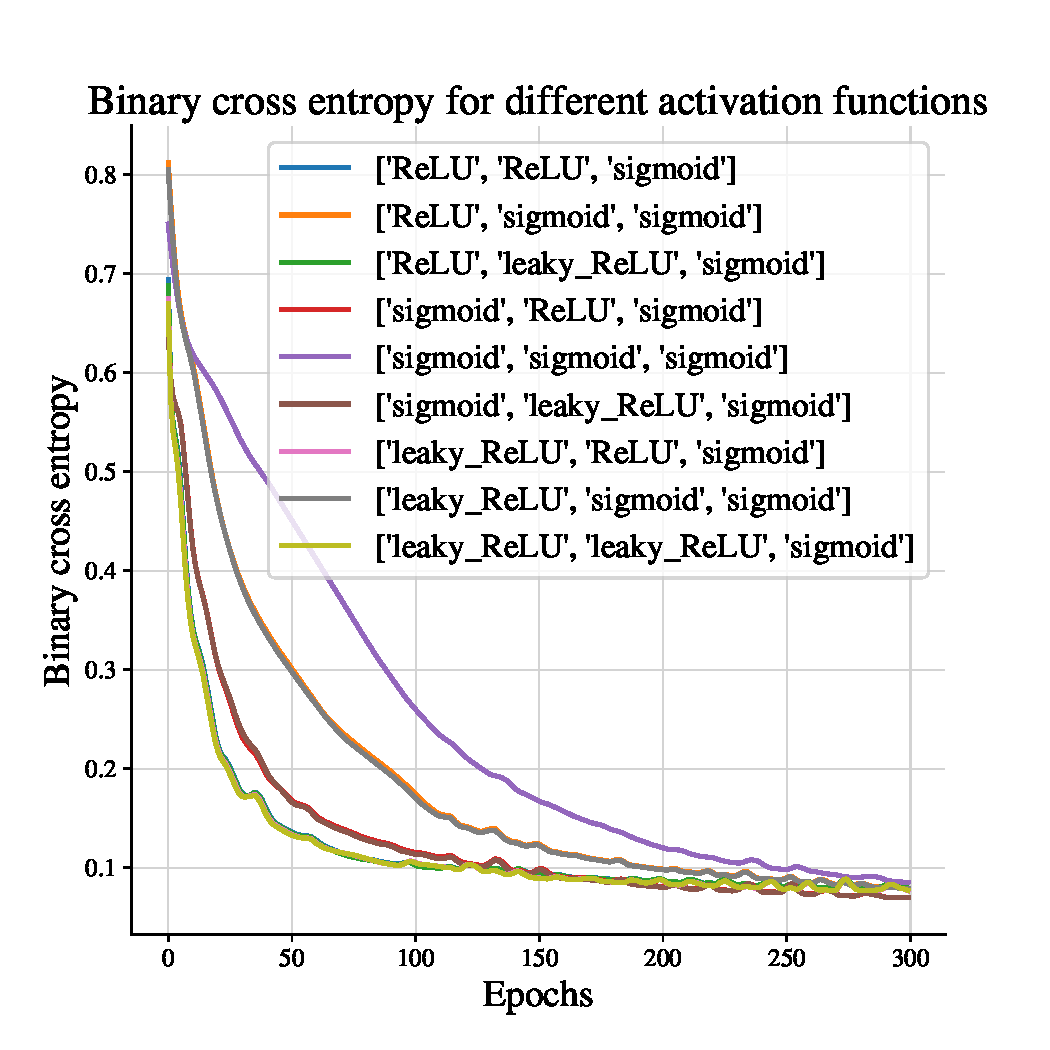
\includegraphics[width=1.0\linewidth]{project_2/figures/Binary cross entropy for different activation functions_classification.pdf}
    \caption{Caption}
    \label{fig:activations_cancer}
\end{figure}

\textbf{Initial learning rate and batch size}

\begin{figure}
    \centering
    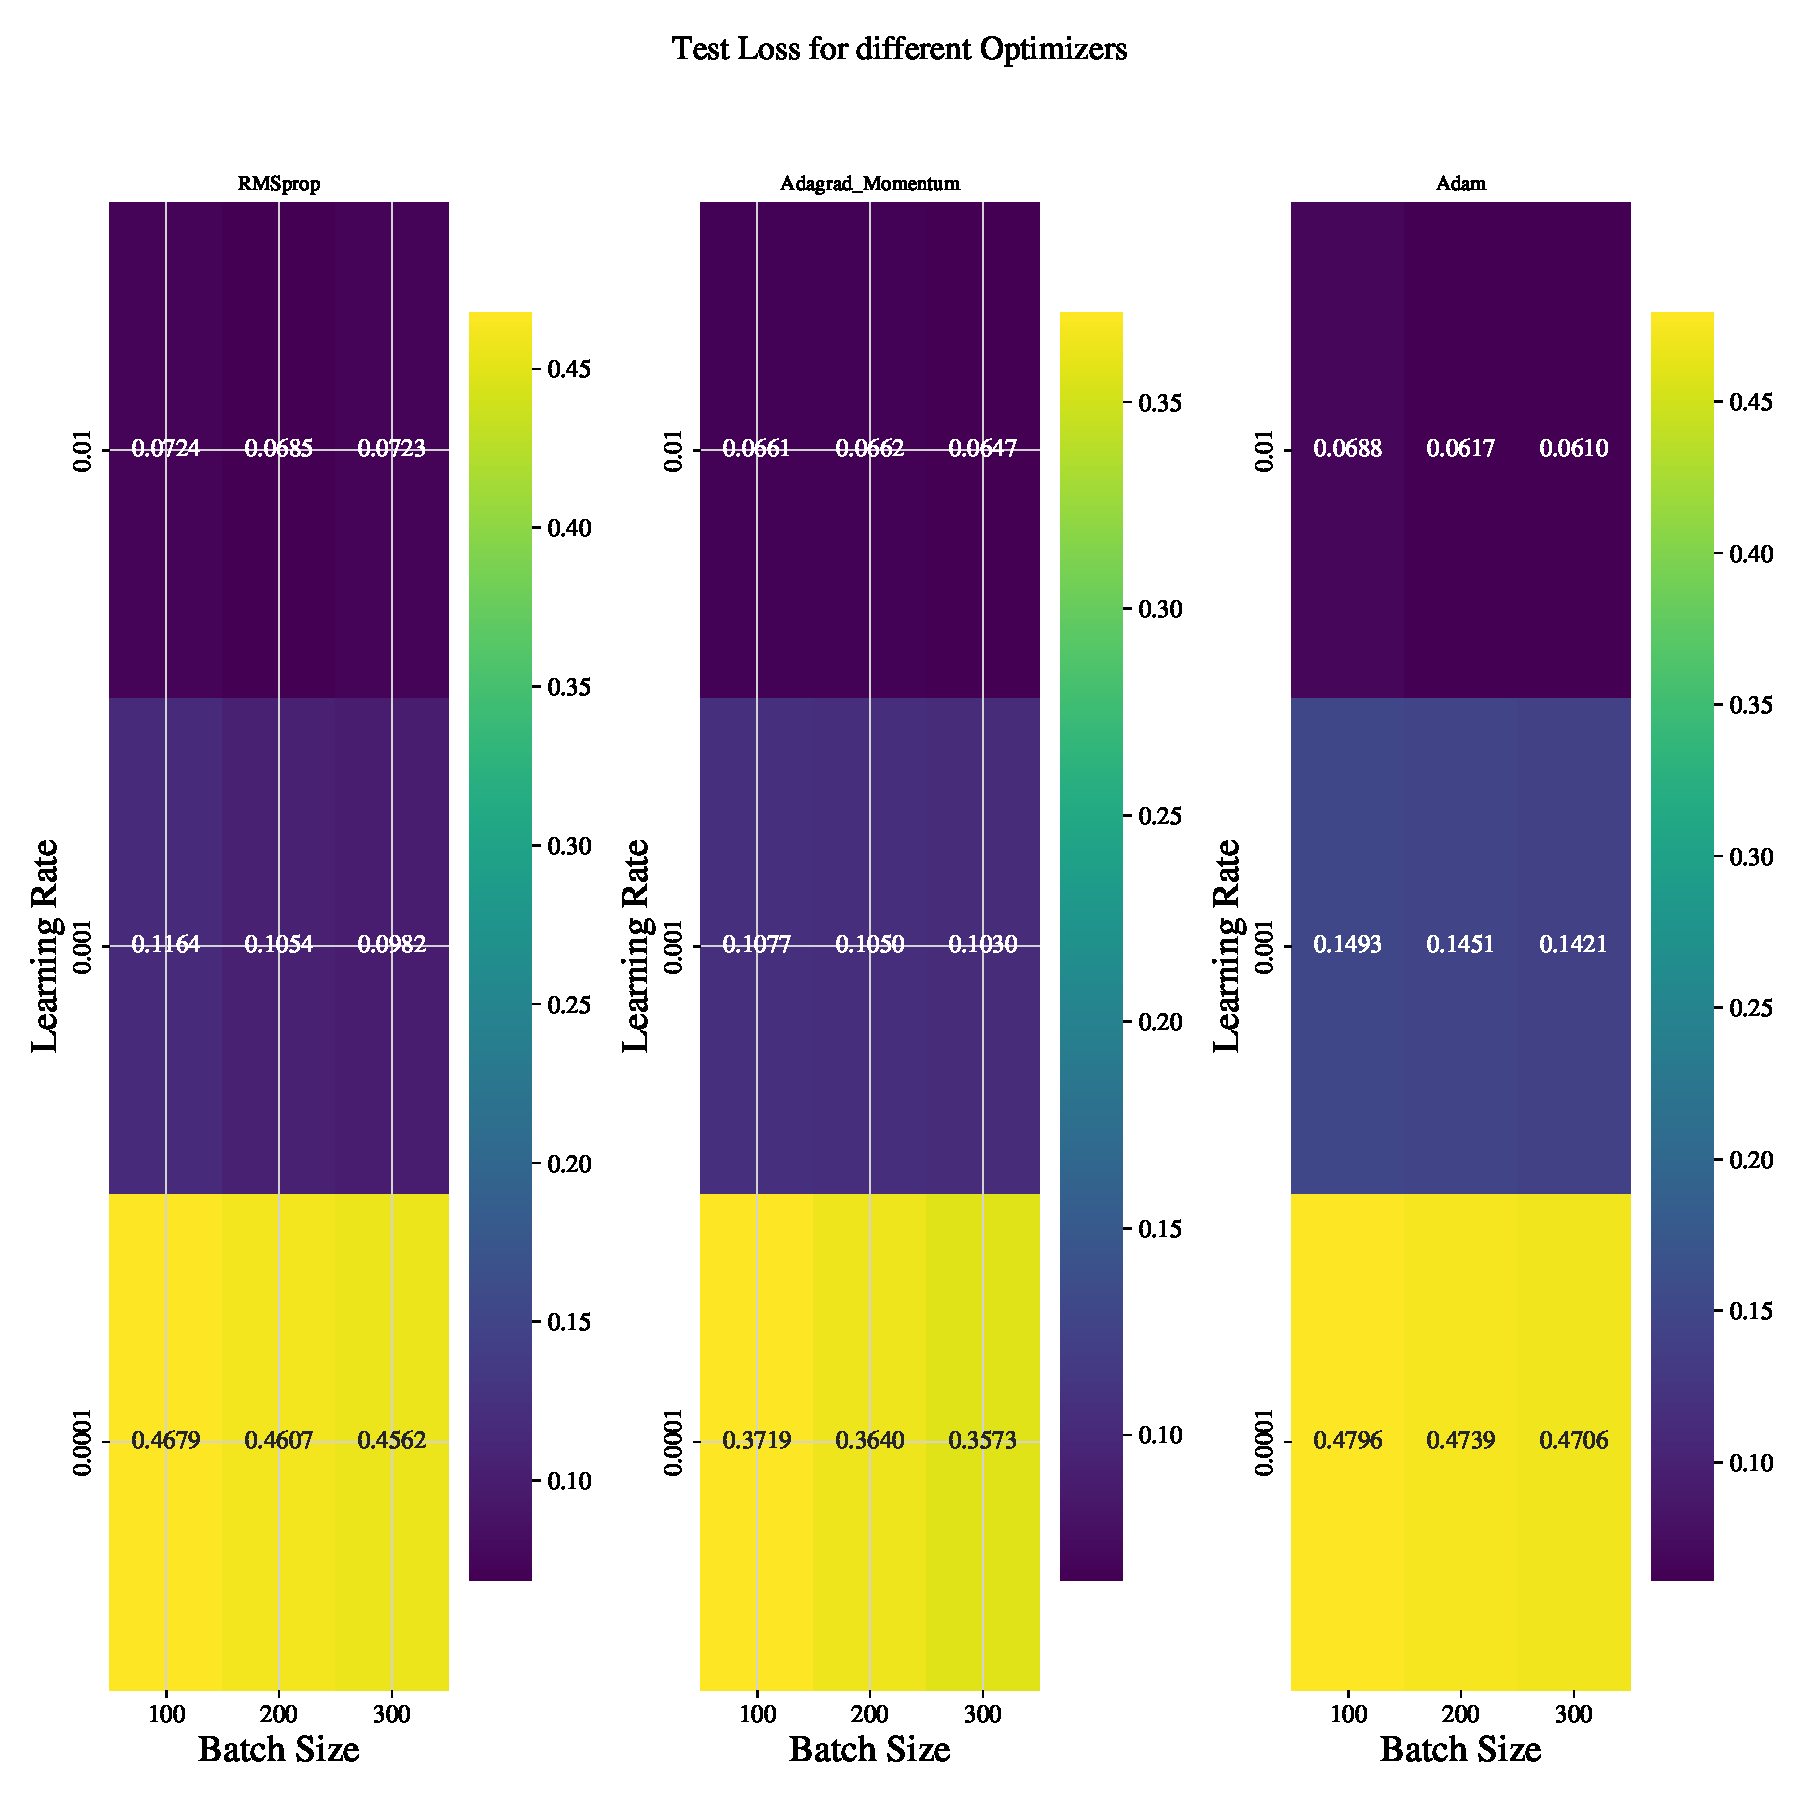
\includegraphics[width=1.0\linewidth]{project_2/figures/Loss_grid_classification.pdf}
    \caption{Caption}
    \label{fig:grid_cancer}
\end{figure}

\textbf{The best model}

\begin{figure}
    \centering
    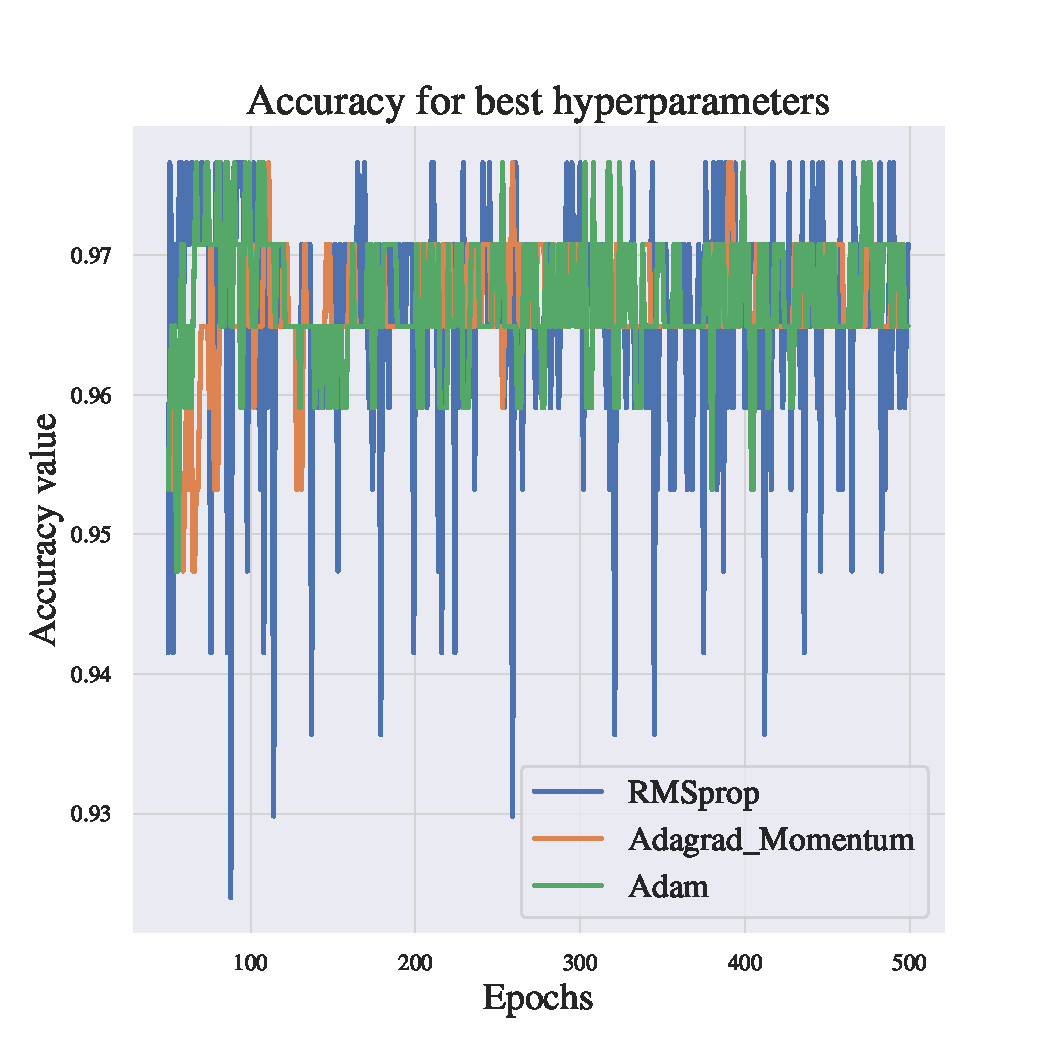
\includegraphics[width=1.0\linewidth]{project_2/figures/best_classification.pdf}
    \caption{Caption}
    \label{fig:best_cancer}
\end{figure}

Final values: 


\subsubsection{Logistic regression}

Final values: 









%Compare the results from the last project with the FFNN for regression tasks (can use Franke function)

%Compare the results from a logistic regression with the FFNN for classification tasks (breast cancer data)

%\mia{Desired plots:
%\begin{itemize}
%    \item Compare the gradient descent methods for OLS
%    \item Compare the gradient descent methods for Ridge
%    \item Compare results from FFNN to project 1 for OLS
%    \item Compare results from FFNN to project 1 for Ridge
%    \item compare logreg to ffnn for OLS and Ridge
%\end{itemize}}

%\mia{Needs discussion:\begin{itemize}
%    \item Learning rate $\eta$
%    \item Number of mini-batches 
%    \item Number of epochs 
%    \item For Ridge: the results as functions of $\lambda$
%    \item lin reg code from project 1 versus ffnn
%    \item critical discussion of pros and cons for each of the methods 
%\end{itemize}}